\documentclass[a4paper,12pt,hidelinks]{apa7}

% PAQUETES
% PAQUETES

% Paquetes de idioma y codificación principales
\usepackage[utf8]{inputenc} % Permite usar caracteres UTF-8.
\usepackage[T1]{fontenc} % Mejora la codificación de las fuentes.
\usepackage{helvet} % Proporciona una fuente compatible con Helvetica.

\usepackage[spanish, es-nodecimaldot]{babel} % Adapta el documento al idioma español.
\usepackage{float}
\usepackage{csquotes} % Gestiona correctamente las comillas.
\usepackage{graphicx} % Permite insertar y ajustar imágenes.
\usepackage{booktabs} % Crea tablas con formato profesional.
\usepackage{bookmark} % Mejora la generación de marcadores PDF.
\usepackage{amsmath} % Añade herramientas para fórmulas matemáticas.
\usepackage[
    backend=biber,
    style=apa
]{biblatex} % Gestiona las referencias bibliográficas en formato APA.

% Paquetes de diseño y formato
\usepackage{xcolor} % Permite definir y usar colores personalizados.
\usepackage{tikz} % Permite crear gráficos y formas vectoriales.
\usepackage{tocloft}[v=2]

% Carga el archivo de referencias bibliográficas.
\addbibresource{bibliography/references.bib}

% METADATOS
% Define el título del documento.
\title{Sistema de Gestión de Tareas}

% Define el título corto para el encabezado.
\shorttitle{Sistema de Gestión de Tareas}

% Define el autor del documento.
\author{Juan Diego Castañeda González}

% Define la afiliación institucional.
\authorsaffiliations{Fundación Universitaria Compensar}

% Define el nombre de la asignatura
\course{Diseño de Software}

% Nombre del profesor
\professor{Nombre del profesor}

% Datos de la fecha de hoy
\duedate{\today}

% CONFIGURACIONES
% Diseño de border y tabla de contenido
\usetikzlibrary{calc} % Facilita cálculos de coordenadas en TikZ.

%\hypersetup{hidelinks} % Configura los enlaces y referencias clicables del PDF. Se agrega en documenclass para mayor comodidad


% No numerar los títulos según la estructura APA
\setcounter{secnumdepth}{-1}

% \setcounter{secnumdepth}{5} % Numeración de secciones

% Profundidad en la tabla de contenido
% \setcounter{tocdepth}{5}

% Puntos de relleno entre el título de la entrada y el número de página
\renewcommand{\cftsecleader}{\cftdotfill{\cftdotsep}} % Títulos
\renewcommand{\cftsubsecleader}{\cftdotfill{\cftdotsep}} % Subsecciones
\renewcommand{\cftsubsubsecleader}{\cftdotfill{\cftdotsep}} % Subsubsecciones

% Eliminar negrilla únicamente en el contenido

\renewcommand{\cftsecfont}{\normalfont} % Títulos
\renewcommand{\cftsubsecfont}{\normalfont} % Subsecciones
\renewcommand{\cftsubsubsecfont}{\normalfont} % Subsubsecciones

% Eliminar negrilla de los números de página

\renewcommand{\cftsecpagefont}{\normalfont} % Títulos
\renewcommand{\cftsubsecpagefont}{\normalfont} % Subsecciones
\renewcommand{\cftsubsubsecpagefont}{\normalfont} % Subsubsecciones


% Centrar el título "Índice" sin someterlo al formato lateral de apa7.
\renewcommand{\cfttoctitlefont}{%
    \hfil
    \bfseries
}
\renewcommand{\cftaftertoctitle}{}

% Define el color naranja institucional.
\definecolor{compensarOrange}{RGB}{255,102,22}
% Define una variante clara del color institucional.
\definecolor{compensarLight}{RGB}{255,190,150}

% Callout
\newtcolorbox{callout}[1][]{
    enhanced,
    breakable,
    colback=gray!5,
    colframe=gray!60,
    boxrule=0.5pt,
    arc=2mm,
    left=3mm,
    right=3mm,
    top=2mm,
    bottom=2mm,
    before skip=10pt,
    after skip=10pt,
    #1
}

\addto\captionsspanish{%
    \renewcommand{\tablename}{Tabla}%
}

\begin{document}
% PORTADA
\begin{titlepage}
    \begin{tikzpicture}[remember picture,overlay]

        % ========================================
        % ESQUINA SUPERIOR IZQUIERDA
        % ========================================
        % ----------------------------------------
        % FRANJA PRIMARIA
        % ----------------------------------------

        \fill[compensarOrange]
        (current page.north west)

        -- ($(current page.north west)+(9cm,0)$)

        .. controls ($(current page.north west)+(6.5cm,-1.2cm)$)
        and ($(current page.north west)+(2.2cm,-5.5cm)$)
        .. ($(current page.north west)+(0,-11cm)$)

        -- cycle;

        % ----------------------------------------
        % FRANJA CLARA / SOMBREADO
        % ----------------------------------------

        \fill[compensarLight, opacity=0.65]

        % Curva exterior:
        % coincide con el borde de la franja primaria
        ($(current page.north west)+(9cm,0)$)

        .. controls ($(current page.north west)+(6.5cm,-1.2cm)$)
        and ($(current page.north west)+(2.2cm,-5.5cm)$)
        .. ($(current page.north west)+(0,-11cm)$)

        % Curva interior:
        % desplazada hacia el centro de la página
        -- ($(current page.north west)+(0,-8.5cm)$)

        .. controls ($(current page.north west)+(2.5cm,-4.5cm)$)
        and ($(current page.north west)+(6cm,-0.8cm)$)
        .. ($(current page.north west)+(11cm,0)$)

        -- cycle;

        % ========================================
        % ESQUINA INFERIOR DERECHA
        % ========================================

        % ----------------------------------------
        % FRANJA PRIMARIA
        % ----------------------------------------

        \fill[compensarOrange]
        (current page.south east)

        -- ($(current page.south east)+(-9cm,0)$)

        .. controls ($(current page.south east)+(-6.5cm,1.2cm)$)
        and ($(current page.south east)+(-2.2cm,5.5cm)$)
        .. ($(current page.south east)+(0,11cm)$)

        -- cycle;

        % ----------------------------------------
        % FRANJA CLARA / SOMBREADO
        % ----------------------------------------

        \fill[compensarLight, opacity=0.65]

        % Curva exterior:
        % coincide con el borde de la franja primaria
        ($(current page.south east)+(-9cm,0)$)

        .. controls ($(current page.south east)+(-6.5cm,1.2cm)$)
        and ($(current page.south east)+(-2.2cm,5.5cm)$)
        .. ($(current page.south east)+(0,11cm)$)

        % Curva interior:
        % desplazada hacia el centro de la página
        -- ($(current page.south east)+(0,8.5cm)$)

        .. controls ($(current page.south east)+(-2.5cm,4.5cm)$)
        and ($(current page.south east)+(-6cm,0.8cm)$)
        .. ($(current page.south east)+(-11cm,0)$)

        -- cycle;

    \end{tikzpicture}

    \centering
    \vspace*{1cm}

    
\includegraphics[width=0.38\textwidth]{./assets/images/logo_ucompensar-2022.jpg}

    \vspace{1.5cm}

    {\large
        Etapa de Contextualización \textendash{} Importancia del diseño de software
        \par}
    \vspace{1.5cm}
    {\large Juan Diego Castañeda González
        \par}
    \vspace{1.5cm}
    {\large Facultad de Ingeniería de Software \\ Fundación Universitaria Compensar
        \par}
    \vspace{1.5cm}
    {\large 2310\textendash{}8B. Patrón de Diseño de Software
        \par}
    \vspace{1.5cm}

    {\large Docente. John Fredy Céspedes Beltrán\par}
    \vspace{1.5cm}
    {\large \today \par}
\end{titlepage}

% Evita que el encabezado de apa7 intente expandir referencias internas
% inexistentes al cambiar de página después de la portada.
\pagestyle{plain}

\tableofcontents

\newpage

\section{Introducción}
Las herramientas digitales hoy en día forman parte de la vida cotidiana para múltiples actividades académicas, como:

\begin{multicols}{2}
    \begin{itemize}
        \item  Consultar bibliografía.
        \item Acceder a aulas virtuales.
        \item Elaborar documentos.
        \item Comunicarse con docentes y compañeros.
        \item Organizar tareas.
        \item Producir contenidos.
    \end{itemize}
\end{multicols}
 
Sin embargo, la disponibilidad de una herramienta no garantiza la finalidad académica clara para que todos los estudiantes tengan las mismas condiciones equivalentes de acceso, habilidades o acompañamiento. Así que, resulta pertinente describir cómo se utilizan estas herramientas en un contexto universitario concreto.

Esta propuesta delimita el estudio a estudiantes universitarios vinculados a instituciones de educación
superior ubicadas en Bogotá, Colombia. Se propone identificar qué herramientas digitales utilizan, con qué
frecuencia, para cuáles actividades académicas y cómo valoran su utilidad. El proyecto no presupone que la
tecnología mejore automáticamente el aprendizaje; busca producir una descripción ordenada de las prácticas
reportadas por los participantes.

El contexto nacional ayuda a explicar la relevancia del tema, aunque no sustituye la información específica de la población universitaria. El Departamento Administrativo Nacional de Estadística \parencite{dane2025entic} reportó que en 2024 el 82,7\% de los hogares de Bogotá tenía conexión a internet, frente al 65,6\% del total nacional. Estas cifras describen hogares y conectividad, no estudiantes universitarios ni uso educativo; por tanto, se emplean únicamente como indicador contextual de acceso.

La \textcite{unesco2023tecnologia} advierte que el potencial educativo de la tecnología depende de cómo se integra a la enseñanza y de las condiciones en que se utiliza. En consecuencia, estudiar la frecuencia, las finalidades y las percepciones de uso puede ofrecer información útil para orientar actividades de alfabetización digital y estrategias de apoyo académico, sin confundir asociación, percepción y causalidad.

\subsection{Delimitación}
La propuesta se centra en estudiantes mayores de edad, matriculados en programas técnicos profesionales, tecnológicos o universitarios de instituciones de educación superior de Bogotá durante el periodo de aplicación que se defina. Como todavía no se ha seleccionado una institución ni se dispone de un marco muestral, el alcance territorial es Bogotá y la selección definitiva de participantes queda condicionada a los permisos y recursos disponibles.

\subsection{Propósito del documento}
Presentar un diseño metodológico viable para una investigación descriptiva, establecer variables
observables y proponer procedimientos de recolección y análisis que puedan ejecutarse después de la aprobación
académica y ética correspondiente.
\section{Planteamiento problema}
El uso de plataformas educativas, buscadores, bibliotecas digitales, procesadores de texto, aplicaciones de
colaboración y asistentes basados en inteligencia artificial se ha diversificado. No obstante, dentro de una
población universitaria pueden existir diferencias en frecuencia, finalidad, percepción de utilidad, habilidades
digitales y dificultades de acceso. Sin datos recogidos de los propios estudiantes, no es posible establecer cuáles
herramientas predominan ni qué barreras son más frecuentes en el grupo concreto que se pretende estudiar.

El problema de investigación consiste en la falta de una caracterización sistemática, para la población
que finalmente se delimite de las herramientas digitales que los estudiantes utilizan con fines académicos, la
frecuencia con que las emplean, sus principales propósitos y las dificultades que reportan. La propuesta no afirma
que exista una magnitud conocida de esta brecha; precisamente plantea medirla mediante un instrumento
estructurado.


\begin{callout}
\textbf{Pregunta de investigación}

¿Qué herramientas digitales utilizan los estudiantes
universitarios de Bogotá, con qué frecuencia y para
qué actividades académicas?
\end{callout}


\begin{figure}[H]
    \caption{Uso de herramientas digitales en estudiantes universitarios de Bogotá, Colombia}
    \label{fig:conectividad-hogares}

    \centering
    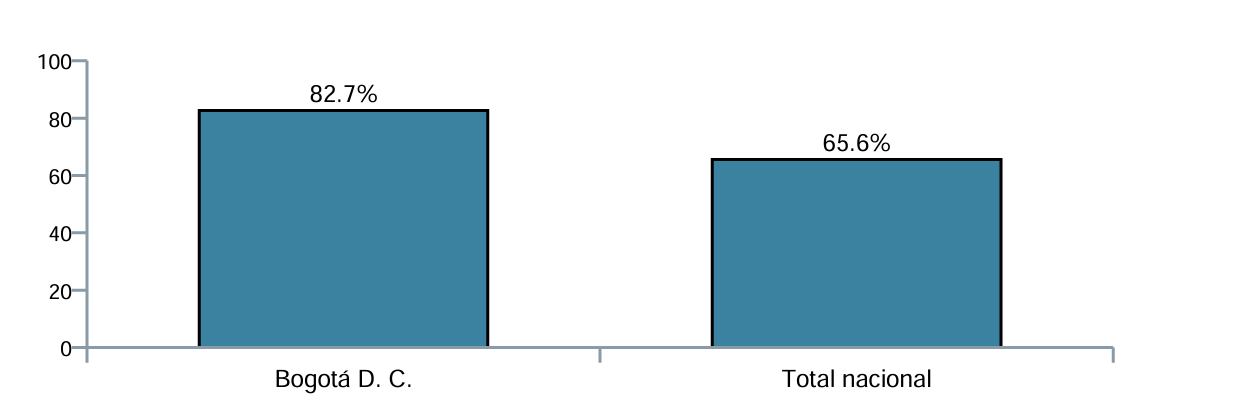
\includegraphics[width=1\textwidth]{assets/images/grafico-conect-Internet.png}

    \par\smallskip
    \begin{minipage}{0.8\textwidth}
        \footnotesize
        \textit{Nota.} Porcentaje de hogares con conexión a internet en 2024. La cifra no corresponde a estudiantes ni mide uso académico. Fuente: DANE \parencite{dane2025entic}, boletín técnico de la ENTIC Hogares 2024.
    \end{minipage}
\end{figure}
\subsection{Justificación del problema}
Una caracterización puede ayudar a reconocer qué herramientas forman parte de las prácticas de estudio,
cuáles se utilizan de manera ocasional y qué dificultades reportan los participantes. Esta información podría servir
como línea base para futuras acciones institucionales; no permitiría, por sí sola, concluir que una herramienta
causa mejores calificaciones o mayor aprendizaje.
\section{Objetivos y justificación}
\subsection{Objetivo general}
Caracterizar el uso de herramientas digitales con fines académicos entre estudiantes universitarios de instituciones de educación superior de Bogotá, considerando los tipos de herramientas utilizadas, la frecuencia, las finalidades y las percepciones de utilidad y dificultad.

\subsection{Objetivos específicos}
\begin{multicols}{2}
    \begin{enumerate}
        \item Identificar las categorías de herramientas digitales que los estudiantes reportan utilizar para realizar actividades académicas.
        \item Describir la frecuencia de uso de las herramientas digitales y las actividades académicas para las que se emplean.
        \vspace{1cm}
        \item Describir la percepción de utilidad y las principales dificultades reportadas en el uso académico de estas herramientas.
        \item Explorar descriptivamente si las respuestas varían según características académicas seleccionadas, como nivel de formación, modalidad de estudio y semestre o periodo cursado, siempre que el tamaño y la composición de la muestra lo permitan.
    \end{enumerate}
\end{multicols}

\subsection{Justificación teórica}
El estudio permite aplicar conceptos metodológicos de investigación a un fenómeno educativo actual. La
UNESCO (2023) plantea que la presencia de tecnología no equivale automáticamente a una transformación
educativa; por eso es necesario analizar prácticas y condiciones de uso, no solo disponibilidad. La investigación
aportaría una descripción situada y podría servir como antecedente para preguntas posteriores más específicas.
\subsection{Justificación práctica}
Los resultados podrían orientar decisiones sobre inducción a plataformas institucionales, uso responsable
de recursos digitales, formación en búsqueda y evaluación de información, colaboración en línea y
acompañamiento a estudiantes que reporten dificultades. Las recomendaciones deberán derivarse de los datos
efectivamente obtenidos y no de expectativas previas del investigador.
\subsection{Justificación social y académica}
La investigación considera que el acceso, la disponibilidad de dispositivos, la conectividad y las
competencias digitales pueden ser desiguales. Aunque el DANE ofrece indicadores agregados de conectividad, el
estudio propuesto se concentra en prácticas universitarias que no quedan descritas por esas cifras generales. La
propuesta puede fomentar una discusión informada sobre inclusión y uso crítico de la tecnología.
\subsection{Viabilidad}
Una encuesta breve en línea o presencial puede aplicarse con recursos limitados, siempre que se obtenga
autorización para contactar participantes y se defina un procedimiento de muestreo transparente. Si no se logra
acceso a varias instituciones, el alcance deberá reducirse explícitamente a la institución o grupo accesible, sin
generalizar a toda Bogotá

\section{Población, muestra y variables}
\subsection{Población objetivo}
Estudiantes de 18 años o más matriculados durante el periodo de estudio en programas de educación superior de instituciones ubicadas en Bogotá, D. C. La definición se plantea para delimitar la propuesta; antes de aplicar el instrumento se debe precisar el periodo académico, los niveles de formación incluidos y las instituciones participantes. Cada estudiante participante que cumpla los criterios de inclusión y responda voluntariamente el cuestionario.
\subsection{Criterios de inclusión y exclusión}
Inclusión: tener 18 años o más, estar matriculado en un programa de educación superior de una institución ubicada en Bogotá y aceptar el consentimiento informado. Exclusión: no cumplir alguno de esos criterios o entregar un cuestionario tan incompleto que impida analizar las variables principales. No se recogerán nombres, documentos de identidad ni contraseñas.
\subsection{Diseño de muestra propuesto}
La opción preferible, si se obtiene un listado de estudiantes y autorización institucional, es un muestreo probabilístico estratificado por institución o nivel de formación, con selección aleatoria dentro de cada estrato. Este procedimiento requiere un marco muestral, información sobre el tamaño de la población y una definición previa de precisión y nivel de confianza. En ausencia de esos elementos no es válido afirmar un tamaño muestral representativo.
Si solo se dispone de participantes voluntarios o de contactos accesibles, se utilizaría una muestra no probabilística por conveniencia, documentando claramente esta limitación. \textcite{argibay2009muestra} discute la diferencia entre muestreo probabilístico y no probabilístico y advierte que la representatividad y la validez externa dependen del procedimiento de selección, no únicamente del número de casos.
\subsection{Tamaño de muestra}
El tamaño definitivo debe calcularse después de conocer el tamaño de la población accesible y decidir el nivel de confianza, el margen de error y la proporción esperada para el indicador principal. Si se emplea una muestra por conveniencia, el número de respuestas se definirá con base en la viabilidad y se reportará como muestra de participantes, sin atribuirle representatividad estadística. En esta fase no se asigna una cifra ficticia.
\newpage
\subsection{Variabilidad e indicadores}
\begin{table}[H]
    \caption{Variables e indicadores propuestos}
    \label{tab:variables-indicadores}
    \begin{tabularx}{\textwidth}{
        >{\raggedright\arraybackslash}p{0.23\textwidth}
        >{\raggedright\arraybackslash}X
        >{\raggedright\arraybackslash}p{0.19\textwidth}
    }
        \toprule
        \textbf{Variable} &
        \textbf{Indicador / operacionalización} &
        \textbf{Tipo de dato} \\
        \midrule

        Herramientas utilizadas &
        Categorías seleccionadas: LMS, buscadores, ofimática, videoconferencia, colaboración, IA y otras. &
        Categórica múltiple \\

        Frecuencia de uso &
        Nunca, rara vez, semanal, varias veces por semana, diariamente. &
        Ordinal \\

        Finalidad académica &
        Consultar fuentes, redactar, practicar, comunicarse, organizar tareas y crear contenidos. &
        Categórica múltiple \\

        Utilidad percibida &
        Escala de respuesta de 1 a 5, de nada útil a muy útil. &
        Ordinal \\

        Dificultades reportadas &
        Conectividad, dispositivo, costo, habilidades, accesibilidad, privacidad y otras. &
        Categórica múltiple \\

        Características académicas &
        Nivel de formación, modalidad y semestre o periodo (opcional). &
        Categórica / ordinal \\
        \bottomrule
    \end{tabularx}

    \begin{minipage}{\textwidth}
        \footnotesize
        \textit{Nota.} Las categorías son una propuesta inicial; deben revisarse mediante juicio experto y prueba piloto antes de la aplicación definitiva.
    \end{minipage}
\end{table}


\section{Enfoque, tipo y diseño metodológico}

\subsection{Enfoque cuantitativo}

Se recomienda el enfoque cuantitativo porque la pregunta de investigación busca describir frecuencias, categorías de herramientas digitales y valoraciones recogidas mediante respuestas estructuradas. Este enfoque permite codificar la información, resumirla mediante tablas y porcentajes y comparar descriptivamente grupos cuando la cantidad y la calidad de los datos lo permitan. La elección del enfoque debe guardar coherencia con el problema, los objetivos y los procedimientos previstos para recolectar y analizar la información \parencite{feriaavila2019dimension,guerrero2015metodologia}.

La recomendación no significa que sea el único enfoque posible. Si el propósito central fuera comprender en profundidad las experiencias personales y los significados atribuidos al uso de estas herramientas, sería pertinente considerar un diseño cualitativo. Si se combinaran mediciones estructuradas y entrevistas, podría plantearse un enfoque mixto.

\subsection{Tipo y alcance}

La investigación será aplicada en su orientación práctica y descriptiva en su alcance. Se considera descriptiva porque pretende caracterizar las prácticas de uso de herramientas digitales con fines académicos, sin probar una intervención ni establecer relaciones causales. Puede incorporar comparaciones exploratorias entre subgrupos; sin embargo, estas deberán presentarse como análisis descriptivos y no como evidencia de causalidad.

\subsection{Diseño no experimental y transversal}

El diseño será no experimental, puesto que no se manipularán deliberadamente las variables ni se asignará a los participantes a tratamientos. Será transversal porque la información se recogerá una sola vez durante un periodo previamente definido. Esta elección resulta viable para una caracterización inicial, aunque no permite observar cambios a lo largo del tiempo ni demostrar que una herramienta produzca mejoras en el rendimiento académico.

\subsection{Método y fases}

El procedimiento metodológico se organizará en seis fases:

\begin{enumerate}
    \item \textbf{Delimitación:} seleccionar la institución o las instituciones participantes, el periodo académico y la población accesible; además, obtener las autorizaciones necesarias.

    \item \textbf{Diseño del instrumento:} elaborar un cuestionario alineado con las variables de estudio y someterlo a revisión para evaluar la claridad y pertinencia de las preguntas.

    \item \textbf{Prueba piloto:} aplicar el cuestionario a un grupo pequeño con características similares a las de la población objetivo, procurando que sus respuestas no se incluyan en el análisis principal cuando sea posible. Ajustar las preguntas ambiguas a partir de los resultados de esta prueba.

    \item \textbf{Recolección de datos:} invitar a los estudiantes a participar voluntariamente, informarles sobre el propósito del estudio y obtener su consentimiento informado.

    \item \textbf{Depuración y análisis:} revisar los registros incompletos, codificar las respuestas y calcular las estadísticas descriptivas correspondientes. La definición de la muestra y su alcance deberán documentarse de manera explícita, especialmente si se recurre a participantes voluntarios \parencite{argibay2009muestra}.

    \item \textbf{Elaboración del informe:} presentar los resultados obtenidos, las limitaciones del estudio y las recomendaciones que se deriven de la evidencia recopilada.
\end{enumerate}

\subsection{Razones para elegir esta metodología}

La metodología propuesta responde directamente a la pregunta de investigación, emplea variables observables y utiliza un instrumento de aplicación relativamente breve. Asimismo, facilita resumir las respuestas de distintos estudiantes y puede ejecutarse con recursos académicos ordinarios.

Su principal limitación es que las respuestas serán autoinformadas y podrían verse afectadas por errores de memoria, interpretaciones diferentes de las opciones o deseabilidad social. La selección muestral también condicionará el alcance de las conclusiones, por lo que deberá distinguirse entre los resultados obtenidos en la muestra y las posibles inferencias hacia una población más amplia \parencite{argibay2009muestra}.

\subsection{Coherencia metodológica}

La correspondencia entre los componentes principales del estudio se establece de la siguiente manera:


\begin{callout}
    \textbf{Coherencia metodológica}
    \smallskip
    \centering
    \textbf{Pregunta descriptiva}
    \(\rightarrow\)
    \textbf{Encuesta estructurada}
    \(\rightarrow\)
    \textbf{Variables observables}
    \(\rightarrow\)
    \textbf{Estadística descriptiva}
    \(\rightarrow\)
    \textbf{Conclusiones delimitadas}
\end{callout}


\section{Técnicas, instrumentos y plan de análisis}

\subsection{Técnica principal: encuesta}

Se propone una encuesta estructurada y autoadministrada, preferiblemente digital y accesible desde computador o teléfono. El instrumento incluirá una explicación breve del estudio, el consentimiento informado, los criterios de inclusión y preguntas sobre las herramientas digitales utilizadas, la frecuencia de uso, las finalidades académicas, la utilidad percibida y las dificultades reportadas.

Las opciones de respuesta deberán redactarse de forma neutral y comprensible. Cuando corresponda, las categorías serán mutuamente excluyentes; en preguntas de selección múltiple se permitirá marcar varias opciones. También se podrán incluir las alternativas \textit{Otra} y \textit{Prefiero no responder} cuando resulten pertinentes.

\subsection{Instrumento: cuestionario}

El cuestionario se organizará en cinco secciones:

\begin{enumerate}
    \item \textbf{Elegibilidad y consentimiento:} verificación de los criterios de inclusión y aceptación voluntaria de la participación.
    
    \item \textbf{Características académicas:} nivel de formación, modalidad de estudio y semestre o periodo cursado, cuando estos datos sean necesarios para los objetivos.
    
    \item \textbf{Herramientas y frecuencia:} identificación de las categorías de herramientas utilizadas y periodicidad de uso.
    
    \item \textbf{Finalidades académicas:} actividades para las que se emplean las herramientas, como consultar fuentes, redactar documentos, comunicarse, colaborar y organizar tareas.
    
    \item \textbf{Utilidad y dificultades:} valoración de la utilidad percibida y registro de barreras relacionadas con conectividad, dispositivos, costos, habilidades, accesibilidad o privacidad.
\end{enumerate}

Se evitarán preguntas que soliciten contraseñas, credenciales de acceso o información personal innecesaria. Antes de la aplicación definitiva, se realizará una prueba piloto para evaluar la comprensión de los ítems, la pertinencia de las opciones de respuesta y el tiempo requerido para completar el cuestionario. Los ajustes se documentarán antes de iniciar la recolección principal.

\subsection{Técnica complementaria: revisión documental}

Se utilizará la revisión documental para contextualizar el fenómeno y fundamentar el marco referencial. Se consultarán fuentes académicas, informes institucionales y documentos normativos pertinentes para el objeto de estudio.

Además, permitirá orientar la comunicación
de los resultados del estudio. La organización clara y concisa de la información científica es relevante para presentar los hallazgos de manera comprensible y estructurada
\parencite{osmarueda2012resumen}.

Esta actividad no se presentará como una revisión sistemática, dado que la propuesta no contempla un protocolo exhaustivo de búsqueda, criterios de elegibilidad registrados ni una evaluación formal del riesgo de sesgo. Las entrevistas no son indispensables para el objetivo descriptivo actual; podrían incorporarse en una fase posterior si se decide profundizar en las experiencias de los estudiantes.



\subsection{Plan de análisis de datos}

El análisis se desarrollará mediante las siguientes etapas:

\begin{enumerate}
    \item \textbf{Depuración:} revisar la elegibilidad de los registros, identificar duplicados detectables y examinar los datos faltantes. No se imputarán automáticamente respuestas ausentes; se documentará el tratamiento aplicado.

    \item \textbf{Codificación:} asignar códigos a las categorías de respuesta y establecer reglas para el procesamiento de preguntas de selección múltiple. Se conservará un registro de las decisiones de codificación para facilitar la trazabilidad del análisis.

    \item \textbf{Estadística descriptiva:} calcular frecuencias absolutas y porcentajes para las herramientas utilizadas, las finalidades académicas y las dificultades reportadas. La frecuencia de uso y la utilidad percibida se resumirán mediante distribuciones por categoría. Las medidas de resumen se elegirán de acuerdo con el nivel de medición de cada variable.

    \item \textbf{Comparación exploratoria:} cruzar variables seleccionadas, por ejemplo, modalidad de estudio y frecuencia de uso, únicamente cuando el número de observaciones por categoría permita una interpretación prudente. Estas comparaciones no se interpretarán como evidencia de causalidad.

    \item \textbf{Presentación de resultados:} elaborar tablas y gráficos con títulos descriptivos, denominadores explícitos y el número de respuestas válidas correspondiente a cada análisis. Se informarán las limitaciones de los datos y las decisiones de procesamiento.
\end{enumerate}

\subsection{Criterios de interpretación}

Los resultados se interpretarán de acuerdo con el procedimiento de selección de la muestra, la calidad de las respuestas y los objetivos descriptivos. La representatividad no se establecerá únicamente a partir del número de participantes, sino considerando el procedimiento de selección y las características del marco muestral \parencite{argibay2009muestra}.

No se anticiparán valores de significación estadística, intervalos de confianza ni asociaciones como si ya se hubieran calculado. Si se selecciona una muestra probabilística y los objetivos lo justifican, podrán definirse procedimientos inferenciales antes del análisis, con la asesoría metodológica correspondiente. En cambio, si se utiliza una muestra por conveniencia, las comparaciones se interpretarán con prudencia y no se generalizarán automáticamente a toda la población universitaria de Bogotá.

\subsection{Consideraciones éticas y protección de datos}

La participación será voluntaria y los estudiantes podrán retirarse sin penalización. Antes de responder, recibirán información sobre la finalidad del estudio, el uso previsto de los datos, su conservación y las personas autorizadas para consultarlos. Se recopilará únicamente la información necesaria y se limitará el acceso a los archivos de trabajo.

Los resultados se presentarán de forma agregada, evitando la divulgación de datos que permitan identificar a los participantes. La Ley 1581 de 2012 establece disposiciones generales para la protección de datos personales en Colombia \parencite{colombia2012ley1581}; por ello, antes de iniciar la recolección se revisarán las obligaciones aplicables y los procedimientos éticos y de protección de datos de la institución participante.

Si se modifica la población para incluir menores de edad, será necesario revisar el protocolo y obtener las autorizaciones y salvaguardas correspondientes antes de su participación.


\section{Marco referencial}

\subsection{Marco teórico}

Las herramientas digitales han adquirido relevancia en los procesos de enseñanza y aprendizaje de la educación superior, al facilitar el acceso a información, la comunicación entre los participantes, la elaboración de contenidos y el desarrollo de actividades académicas. Su incorporación, sin embargo, no garantiza por sí misma una mejora del aprendizaje, pues sus resultados dependen de las condiciones de acceso, las competencias de los usuarios, los objetivos pedagógicos y las formas de utilización.

El Informe de seguimiento de la educación en el mundo de la UNESCO examina las oportunidades y los desafíos de la tecnología en la educación y destaca la importancia de evaluar su pertinencia, equidad y contribución a los objetivos educativos \parencite{unesco2023tecnologia}. Desde esta perspectiva, estudiar el uso de herramientas digitales requiere considerar no solamente su disponibilidad, sino también la frecuencia con la que se utilizan, las actividades para las que se emplean y las dificultades que experimentan los estudiantes.

Para esta investigación, el análisis se orienta hacia una caracterización descriptiva de las prácticas digitales en el contexto universitario. No se parte del supuesto de que utilizar más herramientas implique necesariamente obtener mejores resultados académicos; en cambio, se busca identificar patrones de uso y percepciones que permitan comprender cómo se integran estas tecnologías en las actividades de estudio.

\subsection{Marco conceptual}

Para delimitar el objeto de estudio, se establecen los siguientes conceptos operativos:

\begin{itemize}
    \item \textbf{Herramientas digitales:} aplicaciones, plataformas y servicios tecnológicos que los estudiantes utilizan para desarrollar actividades académicas, como consultar información, elaborar documentos, comunicarse, colaborar o gestionar tareas.

    \item \textbf{Uso académico:} utilización de una herramienta digital con una finalidad vinculada con las actividades de aprendizaje, la elaboración de trabajos, la consulta de fuentes, la comunicación académica o la organización del estudio.

    \item \textbf{Frecuencia de uso:} periodicidad con la que un estudiante utiliza una herramienta para fines académicos. Se medirá mediante categorías ordenadas de respuesta, desde nunca hasta diariamente.

    \item \textbf{Finalidad de uso:} actividad concreta para la cual se emplea una herramienta digital. Se contemplan, entre otras, la búsqueda de información, la redacción, la comunicación, la colaboración y la organización de tareas.

    \item \textbf{Utilidad percibida:} valoración subjetiva que realiza el estudiante sobre la contribución de una herramienta a sus actividades académicas. Se recogerá mediante una escala de respuesta definida en el cuestionario.

    \item \textbf{Barreras de acceso y uso:} dificultades que pueden limitar la utilización de herramientas digitales, como la conectividad, la disponibilidad de dispositivos, los costos, las habilidades digitales, la accesibilidad o las preocupaciones relacionadas con la privacidad.
\end{itemize}

Estas definiciones tienen una finalidad operativa: orientar la construcción del cuestionario, establecer categorías de respuesta y mantener la correspondencia entre los objetivos, las variables y el análisis de los datos. Las categorías definitivas deberán revisarse antes de la aplicación del instrumento.

\subsection{Marco contextual}

La investigación se delimita geográficamente a Bogotá, Distrito Capital, Colombia, y se dirige a estudiantes de 18 años o más matriculados en programas de educación superior de instituciones ubicadas en la ciudad durante el periodo que se establezca para la recolección de información.

Como referencia contextual sobre las condiciones de conectividad, el Departamento Administrativo Nacional de Estadística reportó que, en 2024, el porcentaje de hogares con conexión a internet fue del 82,7\,\% en Bogotá y del 65,6\,\% en el total nacional \parencite{dane2025entic}. Estas cifras permiten contextualizar las condiciones generales de acceso a internet, pero corresponden a hogares y no a estudiantes universitarios. Por tanto, no deben interpretarse como una medición directa de la conectividad individual, de la frecuencia de uso de herramientas digitales ni de las competencias tecnológicas de la población estudiada.

La selección de Bogotá como ámbito territorial permite delimitar la población objetivo y orientar la planificación del trabajo de campo. No obstante, la población accesible dependerá de las instituciones que autoricen el estudio, de los programas académicos incluidos y de la disponibilidad de un marco muestral. Estas condiciones deberán especificarse antes de determinar el tamaño de la muestra y el alcance de las conclusiones.

\subsection{Marco legal}

El proyecto considera, en primer lugar, la Ley 30 de 1992, mediante la cual se organiza el servicio público de la educación superior en Colombia \parencite{colombia1992ley30}. Esta norma constituye un referente general para situar la investigación en el ámbito de la educación superior; su mención no implica que regule específicamente el uso de las herramientas digitales analizadas.

En materia de información personal, se considera la Ley 1581 de 2012, que establece disposiciones generales para la protección de datos personales en Colombia \parencite{colombia2012ley1581}. En consecuencia, el diseño de la encuesta deberá aplicar criterios de minimización de datos, información clara a los participantes, acceso restringido a los registros y presentación agregada de los resultados.

La aplicación concreta de estas disposiciones dependerá de las características del tratamiento de datos y de los procedimientos institucionales aplicables. Antes de iniciar la recolección, se deberán verificar los requisitos de autorización, consentimiento, custodia y conservación de la información, así como las orientaciones éticas de las instituciones participantes.

\subsection{Integración del marco referencial}

Los componentes del marco referencial cumplen funciones complementarias. El marco teórico aporta una perspectiva para comprender las oportunidades y limitaciones de la tecnología en la educación; el conceptual define las variables que serán observadas; el contextual delimita el territorio y presenta información general sobre conectividad; y el legal orienta el tratamiento responsable de la información recopilada.

En conjunto, estos elementos sustentan una investigación descriptiva de enfoque cuantitativo, con diseño no experimental y transversal. Su función es orientar la recolección y la interpretación de los datos, sin sustituir los resultados empíricos que se obtendrán durante el trabajo de campo.


\begin{figure}[H]
    \caption{Delimitación contextual del estudio}
    \label{fig:delimitacion-contextual}

    \centering

    \begin{tikzpicture}[
        bloque/.style={
            draw=black!60,
            rounded corners=2pt,
            align=center,
            text width=5cm,
            minimum height=1.15cm,
            inner sep=8pt,
            font=\small
        },
        flecha/.style={
            -{Stealth[length=2.5mm]},
            thick,
            black!65
        }
    ]

        % Delimitación geográfica y poblacional
        \node[bloque] (ciudad) {
            \textbf{Bogotá, D. C.}
        };

        \node[bloque, below=0.35cm of ciudad] (instituciones) {
            Instituciones de educación superior
        };

        \node[bloque, below=0.35cm of instituciones] (poblacion) {
            Población propuesta: estudiantes de 18 años o más
        };

        % Objeto de estudio
        \node[
            bloque,
            text width=4.2cm,
            minimum height=2.2cm,
            right=1.3cm of instituciones
        ] (objeto) {
            \textbf{Objeto de estudio}\\[4pt]
            Herramientas digitales para fines académicos
        };

        % Relaciones conceptuales
        \draw[flecha] (ciudad) -- (instituciones);
        \draw[flecha] (instituciones) -- (poblacion);
        \draw[flecha] (instituciones.east) -- (objeto.west);

    \end{tikzpicture}

    \par\smallskip
    \begin{minipage}{0.9\textwidth}
        \footnotesize
        \textit{Nota.} Esquema conceptual de delimitación, no mapa cartográfico ni representación de la ubicación exacta de instituciones.
    \end{minipage}
\end{figure}

\newpage
\section{Conclusiones y limitaciones previstas}

La propuesta plantea caracterizar el uso de herramientas digitales entre estudiantes universitarios de Bogotá a partir de un enfoque cuantitativo, alcance descriptivo y diseño no experimental transversal. La encuesta estructurada es congruente con la necesidad de resumir tipos de herramientas, frecuencia, finalidades, utilidad percibida y dificultades reportadas. Esta elección permite una primera aproximación organizada al fenómeno, pero no permite probar relaciones causales ni medir directamente el aprendizaje.

La población y la muestra deben precisarse antes de la aplicación. Para sostener inferencias a una población definida se requiere un marco muestral y un procedimiento probabilístico compatible con los objetivos y recursos. Si solo es posible reclutar participantes voluntarios, el estudio deberá declarar que la muestra es no probabilística y limitar sus conclusiones a las respuestas obtenidas. El tamaño de la muestra no corrige por sí solo un sesgo de selección \parencite{argibay2009muestra}.

La revisión contextual muestra que la conectividad es relevante, pero los indicadores agregados de hogares no sustituyen la medición de experiencias estudiantiles. Por ello, el proyecto separa explícitamente el dato contextual del DANE de la información que deberá producir la encuesta \parencite{dane2025entic}. Del mismo modo, las recomendaciones sobre formación digital o apoyo institucional solo se formularán después de analizar los datos reales.

\subsection{Limitaciones previsibles}

Primero, el autoinforme puede introducir errores de recuerdo y respuestas socialmente deseables. Segundo, la encuesta en línea podría excluir a personas con dificultades de conectividad o acceso, por lo que conviene ofrecer una alternativa accesible si es viable. Tercero, la heterogeneidad entre instituciones y programas puede dificultar las comparaciones. Cuarto, el diseño transversal representa un periodo puntual y no permite identificar cambios ni establecer precedencia temporal. Quinto, el marco muestral y la institución participante todavía no están definidos.

\subsection{Acciones antes de la entrega final o ejecución}

\begin{enumerate}
    \item Completar los datos de portada y confirmar el nombre de la asignatura y del docente.
    \item Definir si se estudiará una institución específica o varias instituciones de Bogotá.
    \item Consultar directamente las lecturas obligatorias y completar los capítulos señalados por el curso, verificando las páginas y los conceptos que se citen.
    \item Obtener la autorización correspondiente y revisar el consentimiento informado.
    \item Revisar el cuestionario con el docente o un experto y efectuar una prueba piloto.
    \item Ajustar el plan de muestreo y análisis a los recursos reales disponibles.
\end{enumerate}

\subsection{Conclusión general}

El valor de este proyecto reside en producir una descripción transparente y metodológicamente delimitada del uso académico de herramientas digitales. Su calidad dependerá de la coherencia entre pregunta, objetivos, variables, muestra e instrumento, así como de la honestidad al informar las limitaciones. No se presentan resultados de campo porque la investigación aún no se ha ejecutado.

\subsection{Síntesis de la propuesta}


\subsection{Anexo breve: ejemplo de preguntas para el cuestionario}

\begin{table}[H]
    \caption{Ejemplo de preguntas para el cuestionario}
    \label{tab:preguntas-cuestionario}

    \small
    \renewcommand{\arraystretch}{1.3}

    \begin{tabularx}{\textwidth}{
        >{\raggedright\arraybackslash}p{0.22\textwidth}
        >{\raggedright\arraybackslash}X
    }
        \toprule
        \textbf{Dimensión} &
        \textbf{Pregunta propuesta} \\
        \midrule

        Herramientas &
        ¿Cuáles de estas herramientas utiliza para estudiar? (Marque todas las que correspondan). \\

        Frecuencia &
        En las últimas cuatro semanas, ¿con qué frecuencia utilizó herramientas digitales para actividades académicas? \\

        Finalidad &
        ¿Para qué actividades las utiliza principalmente? \\

        Utilidad &
        En una escala de 1 a 5, ¿qué tan útiles le resultan para completar sus tareas académicas? \\

        Dificultades &
        ¿Qué dificultades encuentra al utilizarlas? (Puede seleccionar varias). \\

        \bottomrule
    \end{tabularx}

    \vspace{2mm}
    \begin{minipage}{\textwidth}
        \footnotesize
        \textit{Nota.} Estas preguntas son ejemplos iniciales, no un instrumento validado. Deben revisarse y pilotearse antes de su uso.
    \end{minipage}
\end{table}


\newpage
% Referencias
\printbibliography[
    heading=bibintoc,
    title={Referencias}
]

\end{document}